%%%%%%%%%%%%%%%%%%%%%%%%%%%%%%%%%%%%%%%%%
% Lachaise Assignment
% LaTeX Template
% Version 1.0 (26/6/2018)
%
% This template originates from:
% http://www.LaTeXTemplates.com
%
% Authors:
% Marion Lachaise & François Févotte
% Vel (vel@LaTeXTemplates.com)
%
% License:
% CC BY-NC-SA 3.0 (http://creativecommons.org/licenses/by-nc-sa/3.0/)
%
%%%%%%%%%%%%%%%%%%%%%%%%%%%%%%%%%%%%%%%%%

%----------------------------------------------------------------------------------------
%	PACKAGES AND OTHER DOCUMENT CONFIGURATIONS
%----------------------------------------------------------------------------------------

\documentclass{article}

%%%%%%%%%%%%%%%%%%%%%%%%%%%%%%%%%%%%%%%%%
% Lachaise Assignment
% Structure Specification File
% Version 1.0 (26/6/2018)
%
% This template originates from:
% http://www.LaTeXTemplates.com
%
% Authors:
% Marion Lachaise & François Févotte
% Vel (vel@LaTeXTemplates.com)
%
% License:
% CC BY-NC-SA 3.0 (http://creativecommons.org/licenses/by-nc-sa/3.0/)
% 
%%%%%%%%%%%%%%%%%%%%%%%%%%%%%%%%%%%%%%%%%

%----------------------------------------------------------------------------------------
%	PACKAGES AND OTHER DOCUMENT CONFIGURATIONS
%----------------------------------------------------------------------------------------

\usepackage{amsmath,amsfonts,stmaryrd,amssymb} % Math packages

\usepackage{enumerate} % Custom item numbers for enumerations

\usepackage[ruled]{algorithm2e} % Algorithms

\usepackage[framemethod=tikz]{mdframed} % Allows defining custom boxed/framed environments

\usepackage{listings} % File listings, with syntax highlighting
\lstset{
	basicstyle=\ttfamily, % Typeset listings in monospace font
}

%----------------------------------------------------------------------------------------
%	DOCUMENT MARGINS
%----------------------------------------------------------------------------------------

\usepackage{geometry} % Required for adjusting page dimensions and margins

\geometry{
	paper=a4paper, % Paper size, change to letterpaper for US letter size
	top=2.5cm, % Top margin
	bottom=3cm, % Bottom margin
	left=2.5cm, % Left margin
	right=2.5cm, % Right margin
	headheight=14pt, % Header height
	footskip=1.5cm, % Space from the bottom margin to the baseline of the footer
	headsep=1.2cm, % Space from the top margin to the baseline of the header
	%showframe, % Uncomment to show how the type block is set on the page
}

%----------------------------------------------------------------------------------------
%	FONTS
%----------------------------------------------------------------------------------------

\usepackage[utf8]{inputenc} % Required for inputting international characters
\usepackage[T1]{fontenc} % Output font encoding for international characters

\usepackage{XCharter} % Use the XCharter fonts

%----------------------------------------------------------------------------------------
%	COMMAND LINE ENVIRONMENT
%----------------------------------------------------------------------------------------

% Usage:
% \begin{commandline}
%	\begin{verbatim}
%		$ ls
%		
%		Applications	Desktop	...
%	\end{verbatim}
% \end{commandline}

\mdfdefinestyle{commandline}{
	leftmargin=10pt,
	rightmargin=10pt,
	innerleftmargin=15pt,
	middlelinecolor=black!50!white,
	middlelinewidth=2pt,
	frametitlerule=false,
	backgroundcolor=black!5!white,
	frametitle={Command Line},
	frametitlefont={\normalfont\sffamily\color{white}\hspace{-1em}},
	frametitlebackgroundcolor=black!50!white,
	nobreak,
}

% Define a custom environment for command-line snapshots
\newenvironment{commandline}{
	\medskip
	\begin{mdframed}[style=commandline]
}{
	\end{mdframed}
	\medskip
}

%----------------------------------------------------------------------------------------
%	FILE CONTENTS ENVIRONMENT
%----------------------------------------------------------------------------------------

% Usage:
% \begin{file}[optional filename, defaults to "File"]
%	File contents, for example, with a listings environment
% \end{file}

\mdfdefinestyle{file}{
	innertopmargin=1.6\baselineskip,
	innerbottommargin=0.8\baselineskip,
	topline=false, bottomline=false,
	leftline=false, rightline=false,
	leftmargin=2cm,
	rightmargin=2cm,
	singleextra={%
		\draw[fill=black!10!white](P)++(0,-1.2em)rectangle(P-|O);
		\node[anchor=north west]
		at(P-|O){\ttfamily\mdfilename};
		%
		\def\l{3em}
		\draw(O-|P)++(-\l,0)--++(\l,\l)--(P)--(P-|O)--(O)--cycle;
		\draw(O-|P)++(-\l,0)--++(0,\l)--++(\l,0);
	},
	nobreak,
}

% Define a custom environment for file contents
\newenvironment{file}[1][File]{ % Set the default filename to "File"
	\medskip
	\newcommand{\mdfilename}{#1}
	\begin{mdframed}[style=file]
}{
	\end{mdframed}
	\medskip
}

%----------------------------------------------------------------------------------------
%	NUMBERED QUESTIONS ENVIRONMENT
%----------------------------------------------------------------------------------------

% Usage:
% \begin{question}[optional title]
%	Question contents
% \end{question}

\mdfdefinestyle{question}{
	innertopmargin=1.2\baselineskip,
	innerbottommargin=0.8\baselineskip,
	roundcorner=5pt,
	nobreak,
	singleextra={%
		\draw(P-|O)node[xshift=1em,anchor=west,fill=white,draw,rounded corners=5pt]{%
		Question \theQuestion\questionTitle};
	},
}

\newcounter{Question} % Stores the current question number that gets iterated with each new question

% Define a custom environment for numbered questions
\newenvironment{question}[1][\unskip]{
	\bigskip
	\stepcounter{Question}
	\newcommand{\questionTitle}{~#1}
	\begin{mdframed}[style=question]
}{
	\end{mdframed}
	\medskip
}

%----------------------------------------------------------------------------------------
%	WARNING TEXT ENVIRONMENT
%----------------------------------------------------------------------------------------

% Usage:
% \begin{warn}[optional title, defaults to "Warning:"]
%	Contents
% \end{warn}

\mdfdefinestyle{warning}{
	topline=false, bottomline=false,
	leftline=false, rightline=false,
	nobreak,
	singleextra={%
		\draw(P-|O)++(-0.5em,0)node(tmp1){};
		\draw(P-|O)++(0.5em,0)node(tmp2){};
		\fill[black,rotate around={45:(P-|O)}](tmp1)rectangle(tmp2);
		\node at(P-|O){\color{white}\scriptsize\bf !};
		\draw[very thick](P-|O)++(0,-1em)--(O);%--(O-|P);
	}
}

% Define a custom environment for warning text
\newenvironment{warn}[1][Warning:]{ % Set the default warning to "Warning:"
	\medskip
	\begin{mdframed}[style=warning]
		\noindent{\textbf{#1}}
}{
	\end{mdframed}
}

%----------------------------------------------------------------------------------------
%	INFORMATION ENVIRONMENT
%----------------------------------------------------------------------------------------

% Usage:
% \begin{info}[optional title, defaults to "Info:"]
% 	contents
% 	\end{info}

\mdfdefinestyle{info}{%
	topline=false, bottomline=false,
	leftline=false, rightline=false,
	nobreak,
	singleextra={%
		\fill[black](P-|O)circle[radius=0.4em];
		\node at(P-|O){\color{white}\scriptsize\bf i};
		\draw[very thick](P-|O)++(0,-0.8em)--(O);%--(O-|P);
	}
}

% Define a custom environment for information
\newenvironment{info}[1][Info:]{ % Set the default title to "Info:"
	\medskip
	\begin{mdframed}[style=info]
		\noindent{\textbf{#1}}
}{
	\end{mdframed}
}
 % Include the file specifying the document structure and custom commands

%----------------------------------------------------------------------------------------
%	ASSIGNMENT INFORMATION
%----------------------------------------------------------------------------------------

\title{COMP9417: Homework Set \#1} % Title of the assignment

\author{z5113817} % Author name and email address

\date{University of New South Wales --- \today} % University, school and/or department name(s) and a date

\newcommand\simplelrg{\hat{\beta}_{1} = \frac{\bar{XY} - \bar{X}\bar{Y}}{\bar{(X^2)} - (\bar{X})^2}}

\newcommand\sumlrg{\frac{1}{n}\sum_{i=1}^{n}(}
\newcommand\expandedlrg{\hat{\beta}_{1} = \frac{\sumlrg{}X_{i} - \bar{X})(Y_{i} - \bar{Y})}{\sumlrg{}X_{i} - \bar{X})^2}}

%----------------------------------------------------------------------------------------

\begin{document}

\maketitle % Print the title

%----------------------------------------------------------------------------------------
%	Main Contents
%----------------------------------------------------------------------------------------

\section*{Question 1}

\subsection*{a)}

We know from the normal equations for a the gradient of a minimised linear regression is:

\begin{equation*}
	\simplelrg{}
\end{equation*}

Which can expand into:

\begin{equation*}
	\expandedlrg{}
\end{equation*}

So now substituting in the transformation, we get:

\begin{equation}
	\hat{\beta}_{1} = \frac{\sumlrg{}\tilde{X}_{i} - \bar{X})(Y_{i} - \bar{Y})}{\sumlrg{}\tilde{X}_{i} - \bar{X})^2}
\end{equation}
\begin{equation}
	\hat{\beta}_{1} = \frac{\sumlrg{}c(X_{i} + d) - \bar{X})(Y_{i} - \bar{Y})}{\sumlrg{}c(X_{i} + d) - \bar{X})^2}
\end{equation}
\begin{equation}
	...
\end{equation}

\subsection*{b)}

\newpage
\section*{Question 2}

See Github repository \href{https://github.com/william-coulter/COMP9417_Homework_1/tree/master/python}{here} for all of the python code used in this question.

\subsection*{a)}
\begin{verbatim}
	import pandas as pd
	import seaborn as sns
	import matplotlib.pyplot as plt
	
	df = pd.read_csv("./data/data.csv")
	sns.pairplot(df)
	plt.savefig("./outputs/q2a_pairplots.png")
\end{verbatim}
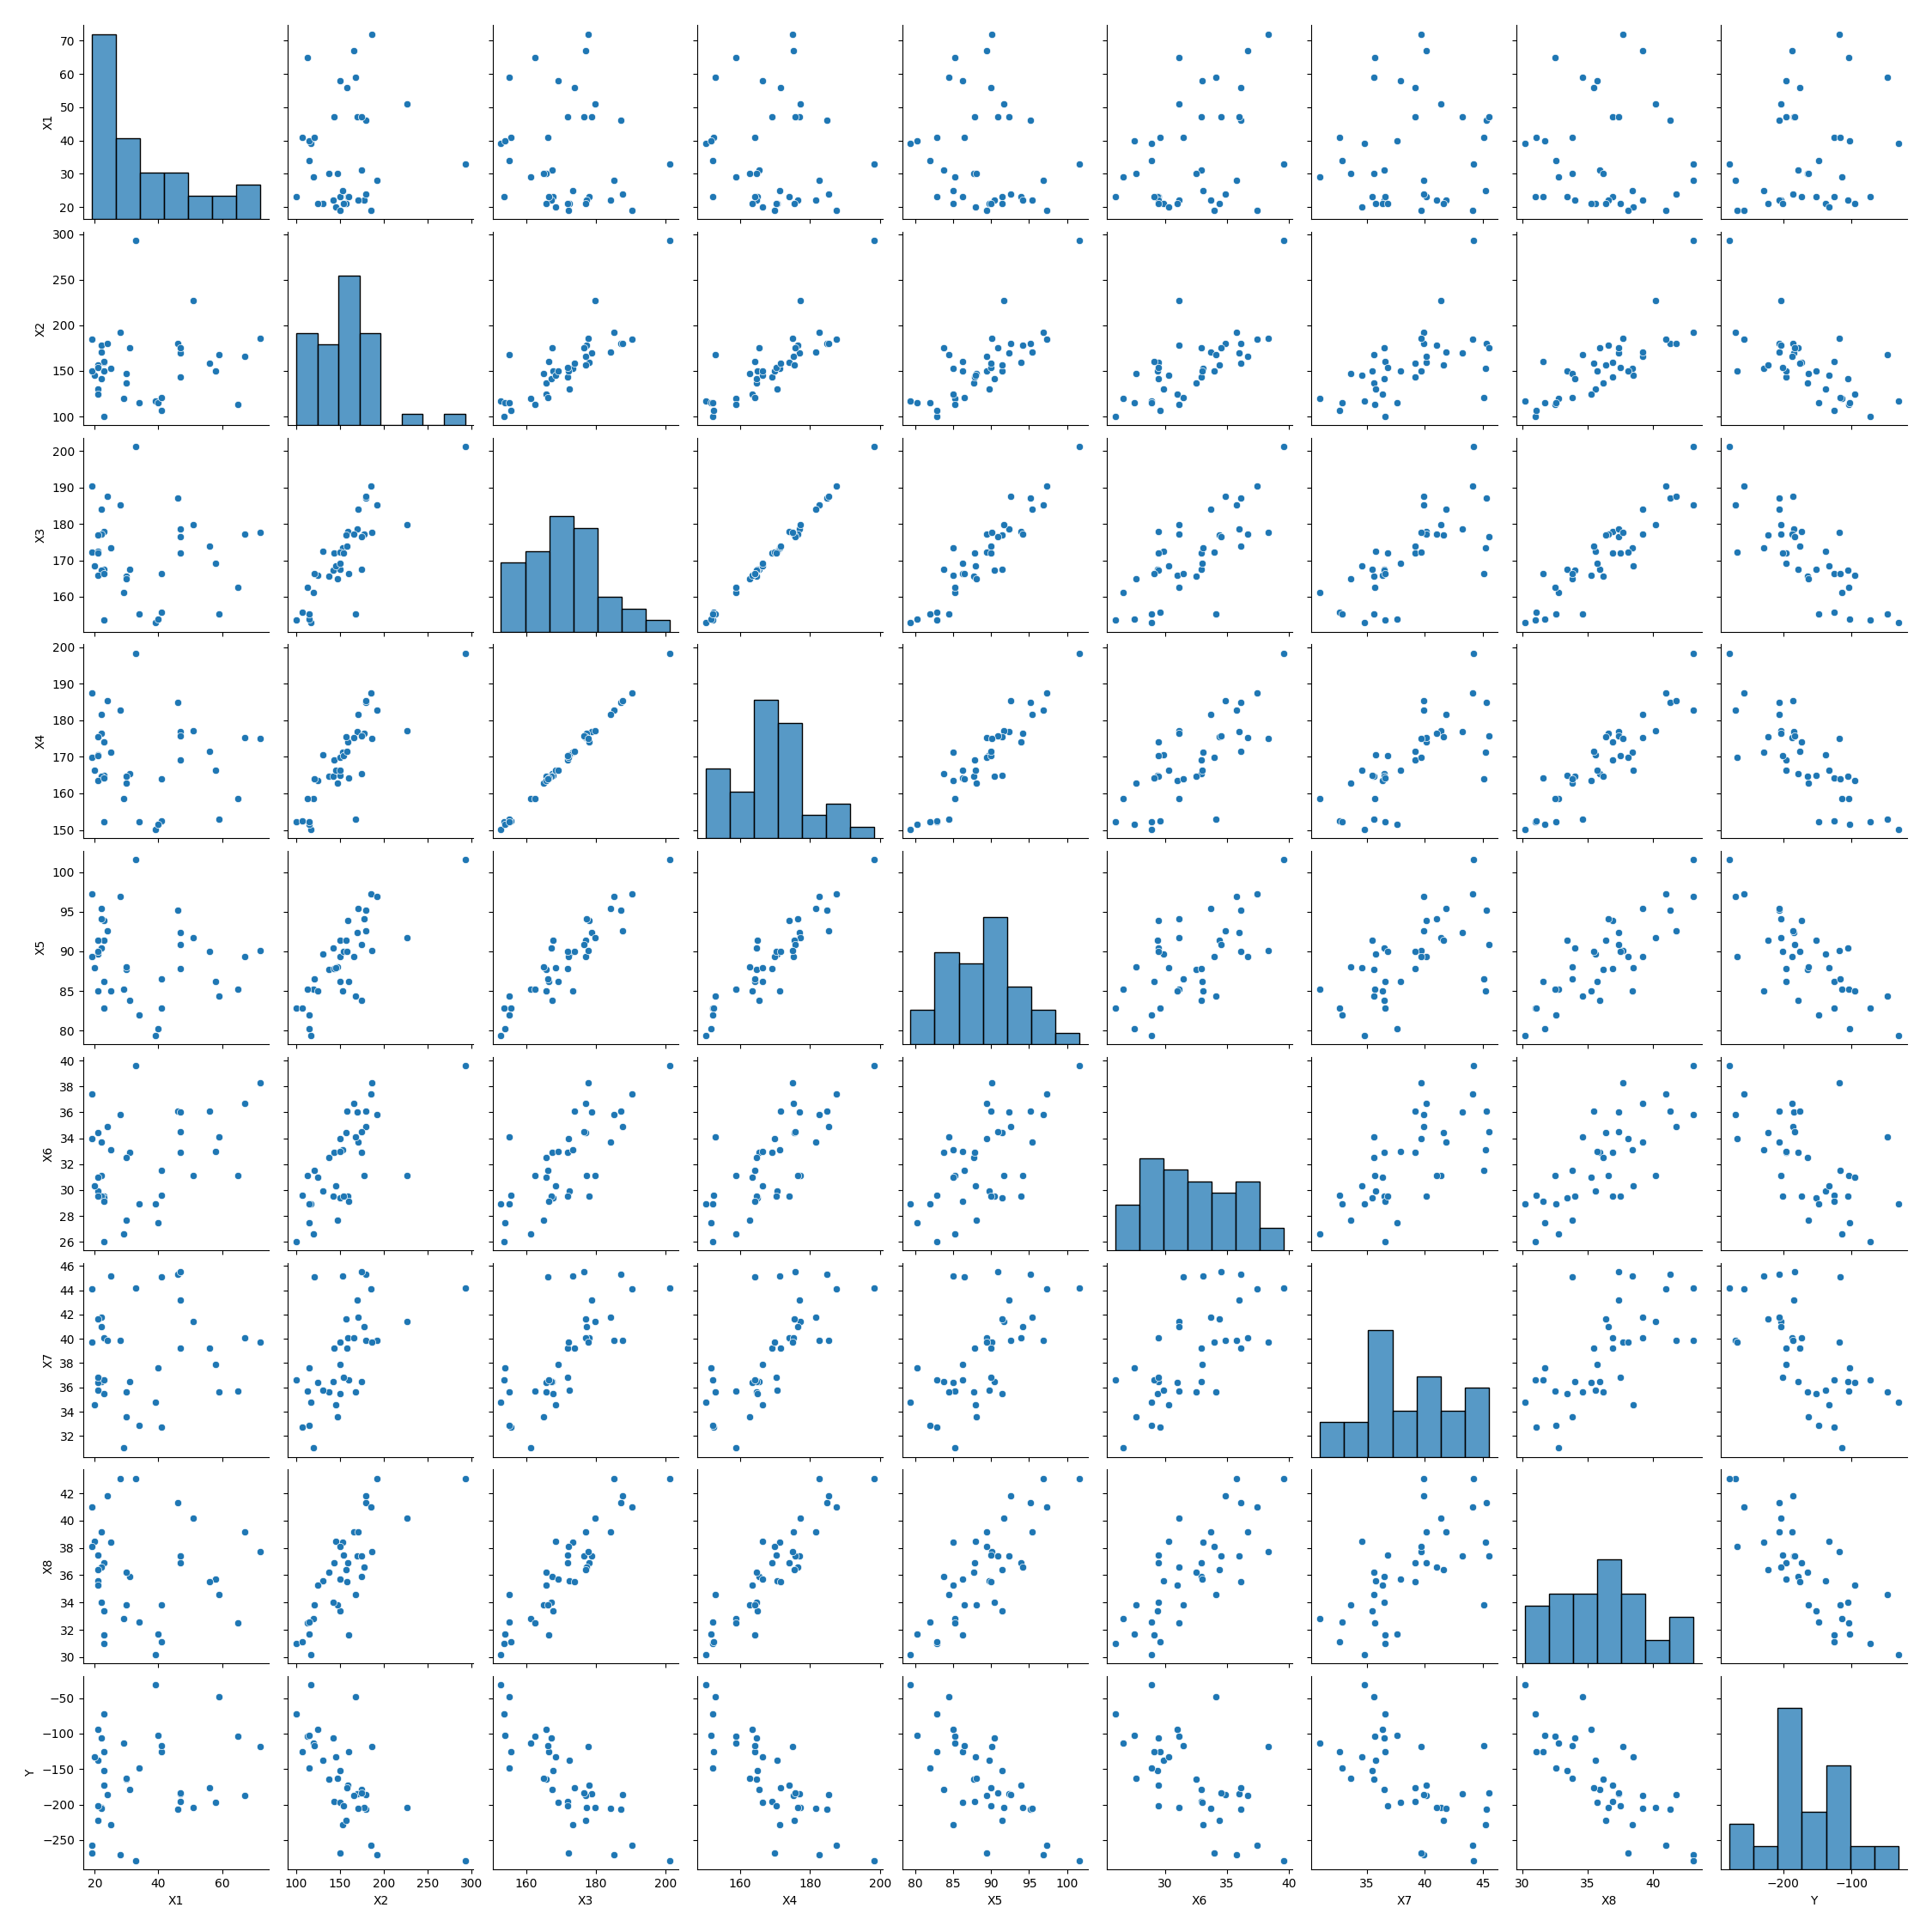
\includegraphics[scale=0.270]{q2a_pairplots.png}

The pairs plots shows a scatter plots between variables in the dataset, while
the histogram on the diagonal shows the distribution of each variable. 
For example, the plot on the fourth row in the second column is the scatter plot of X3
on the y-axis and X2 on the x-axis. Such a matrix is useful for seeing correlations between 
variables. This is important in linear regression to prevent multicollinearity between the 
variables, which can skew the coefficients of the regression model and lead to unreliable
statistical inferences.

\newpage
\subsection*{b)}

The code in \textbf{q2b.py} will produce:

\begin{verbatim}
	Sum of squares for each transformed feature:
	X1: 38.000000000000014
	X2: 38.0
	X3: 38.000000000000014
	X4: 37.999999999999986
	X5: 37.99999999999998
	X6: 38.0
	X7: 38.00000000000001
	X8: 37.999999999999986
\end{verbatim}

These should all be 38 exactly however they are not due to floating point errors.

\subsection*{c)}



%%%%%%%%%%%%%%%%%%%%%


% \begin{info} % Information block
% 	This is an interesting piece of information, to which the reader should pay special attention. Fusce varius orci ac magna dapibus porttitor. In tempor leo a neque bibendum sollicitudin. Nulla pretium fermentum nisi, eget sodales magna facilisis eu. Praesent aliquet nulla ut bibendum lacinia. Donec vel mauris vulputate, commodo ligula ut, egestas orci. Suspendisse commodo odio sed hendrerit lobortis. Donec finibus eros erat, vel ornare enim mattis et.
% \end{info}

%----------------------------------------------------------------------------------------
%	PROBLEM 1
%----------------------------------------------------------------------------------------

% \section{Problem title} % Numbered section

% In hac habitasse platea dictumst. Curabitur mattis elit sit amet justo luctus vestibulum. In hac habitasse platea dictumst. Pellentesque lobortis justo enim, a condimentum massa tempor eu. Ut quis nulla a quam pretium eleifend nec eu nisl. Nam cursus porttitor eros, sed luctus ligula convallis quis. Nam convallis, ligula in auctor euismod, ligula mauris fringilla tellus, et egestas mauris odio eget diam. Praesent sodales in ipsum eu dictum.

% %------------------------------------------------

% \subsection{Theoretical viewpoint}

% Maecenas consectetur metus at tellus finibus condimentum. Proin arcu lectus, ultrices non tincidunt et, tincidunt ut quam. Integer luctus posuere est, non maximus ante dignissim quis. Nunc a cursus erat. Curabitur suscipit nibh in tincidunt sagittis. Nam malesuada vestibulum quam id gravida. Proin ut dapibus velit. Vestibulum eget quam quis ipsum semper convallis. Duis consectetur nibh ac diam dignissim, id condimentum enim dictum. Nam aliquet ligula eu magna pellentesque, nec sagittis leo lobortis. Aenean tincidunt dignissim egestas. Morbi efficitur risus ante, id tincidunt odio pulvinar vitae.

% Curabitur tempus hendrerit nulla. Donec faucibus lobortis nibh pharetra sagittis. Sed magna sem, posuere eget sem vitae, finibus consequat libero. Cras aliquet sagittis erat ut semper. Aenean vel enim ipsum. Fusce ut felis at eros sagittis bibendum mollis lobortis libero. Donec laoreet nisl vel risus lacinia elementum non nec lacus. Nullam luctus, nulla volutpat ultricies ultrices, quam massa placerat augue, ut fringilla urna lectus nec nibh. Vestibulum efficitur condimentum orci a semper. Pellentesque ut metus pretium lacus maximus semper. Sed tellus augue, consectetur rhoncus eleifend vel, imperdiet nec turpis. Nulla ligula ante, malesuada quis orci a, ultricies blandit elit.

% % Numbered question, with subquestions in an enumerate environment
% \begin{question}
% 	Quisque ullamcorper placerat ipsum. Cras nibh. Morbi vel justo vitae lacus tincidunt ultrices. Lorem ipsum dolor sit amet, consectetuer adipiscing elit.

% 	% Subquestions numbered with letters
% 	\begin{enumerate}[(a)]
% 		\item Do this.
% 		\item Do that.
% 		\item Do something else.
% 	\end{enumerate}
% \end{question}

% %------------------------------------------------

% \subsection{Algorithmic issues}

% In malesuada ullamcorper urna, sed dapibus diam sollicitudin non. Donec elit odio, accumsan ac nisl a, tempor imperdiet eros. Donec porta tortor eu risus consequat, a pharetra tortor tristique. Morbi sit amet laoreet erat. Morbi et luctus diam, quis porta ipsum. Quisque libero dolor, suscipit id facilisis eget, sodales volutpat dolor. Nullam vulputate interdum aliquam. Mauris id convallis erat, ut vehicula neque. Sed auctor nibh et elit fringilla, nec ultricies dui sollicitudin. Vestibulum vestibulum luctus metus venenatis facilisis. Suspendisse iaculis augue at vehicula ornare. Sed vel eros ut velit fermentum porttitor sed sed massa. Fusce venenatis, metus a rutrum sagittis, enim ex maximus velit, id semper nisi velit eu purus.

% \begin{center}
% 	\begin{minipage}{0.5\linewidth} % Adjust the minipage width to accomodate for the length of algorithm lines
% 		\begin{algorithm}[H]
% 			\KwIn{$(a, b)$, two floating-point numbers}  % Algorithm inputs
% 			\KwResult{$(c, d)$, such that $a+b = c + d$} % Algorithm outputs/results
% 			\medskip
% 			\If{$\vert b\vert > \vert a\vert$}{
% 				exchange $a$ and $b$ \;
% 			}
% 			$c \leftarrow a + b$ \;
% 			$z \leftarrow c - a$ \;
% 			$d \leftarrow b - z$ \;
% 			{\bf return} $(c,d)$ \;
% 			\caption{\texttt{FastTwoSum}} % Algorithm name
% 			\label{alg:fastTwoSum}   % optional label to refer to
% 		\end{algorithm}
% 	\end{minipage}
% \end{center}

% Fusce varius orci ac magna dapibus porttitor. In tempor leo a neque bibendum sollicitudin. Nulla pretium fermentum nisi, eget sodales magna facilisis eu. Praesent aliquet nulla ut bibendum lacinia. Donec vel mauris vulputate, commodo ligula ut, egestas orci. Suspendisse commodo odio sed hendrerit lobortis. Donec finibus eros erat, vel ornare enim mattis et.

% % Numbered question, with an optional title
% \begin{question}[\itshape (with optional title)]
% 	In congue risus leo, in gravida enim viverra id. Donec eros mauris, bibendum vel dui at, tempor commodo augue. In vel lobortis lacus. Nam ornare ullamcorper mauris vel molestie. Maecenas vehicula ornare turpis, vitae fringilla orci consectetur vel. Nam pulvinar justo nec neque egestas tristique. Donec ac dolor at libero congue varius sed vitae lectus. Donec et tristique nulla, sit amet scelerisque orci. Maecenas a vestibulum lectus, vitae gravida nulla. Proin eget volutpat orci. Morbi eu aliquet turpis. Vivamus molestie urna quis tempor tristique. Proin hendrerit sem nec tempor sollicitudin.
% \end{question}

% Mauris interdum porttitor fringilla. Proin tincidunt sodales leo at ornare. Donec tempus magna non mauris gravida luctus. Cras vitae arcu vitae mauris eleifend scelerisque. Nam sem sapien, vulputate nec felis eu, blandit convallis risus. Pellentesque sollicitudin venenatis tincidunt. In et ipsum libero. Nullam tempor ligula a massa convallis pellentesque.

% %----------------------------------------------------------------------------------------
% %	PROBLEM 2
% %----------------------------------------------------------------------------------------

% \section{Implementation}

% Proin lobortis efficitur dictum. Pellentesque vitae pharetra eros, quis dignissim magna. Sed tellus leo, semper non vestibulum vel, tincidunt eu mi. Aenean pretium ut velit sed facilisis. Ut placerat urna facilisis dolor suscipit vehicula. Ut ut auctor nunc. Nulla non massa eros. Proin rhoncus arcu odio, eu lobortis metus sollicitudin eu. Duis maximus ex dui, id bibendum diam dignissim id. Aliquam quis lorem lorem. Phasellus sagittis aliquet dolor, vulputate cursus dolor convallis vel. Suspendisse eu tellus feugiat, bibendum lectus quis, fermentum nunc. Nunc euismod condimentum magna nec bibendum. Curabitur elementum nibh eu sem cursus, eu aliquam leo rutrum. Sed bibendum augue sit amet pharetra ullamcorper. Aenean congue sit amet tortor vitae feugiat.

% In congue risus leo, in gravida enim viverra id. Donec eros mauris, bibendum vel dui at, tempor commodo augue. In vel lobortis lacus. Nam ornare ullamcorper mauris vel molestie. Maecenas vehicula ornare turpis, vitae fringilla orci consectetur vel. Nam pulvinar justo nec neque egestas tristique. Donec ac dolor at libero congue varius sed vitae lectus. Donec et tristique nulla, sit amet scelerisque orci. Maecenas a vestibulum lectus, vitae gravida nulla. Proin eget volutpat orci. Morbi eu aliquet turpis. Vivamus molestie urna quis tempor tristique. Proin hendrerit sem nec tempor sollicitudin.

% % File contents
% \begin{file}[hello.py]
% \begin{lstlisting}[language=Python]
% #! /usr/bin/python

% import sys
% sys.stdout.write("Hello World!\n")
% \end{lstlisting}
% \end{file}

% Fusce eleifend porttitor arcu, id accumsan elit pharetra eget. Mauris luctus velit sit amet est sodales rhoncus. Donec cursus suscipit justo, sed tristique ipsum fermentum nec. Ut tortor ex, ullamcorper varius congue in, efficitur a tellus. Vivamus ut rutrum nisi. Phasellus sit amet enim efficitur, aliquam nulla id, lacinia mauris. Quisque viverra libero ac magna maximus efficitur. Interdum et malesuada fames ac ante ipsum primis in faucibus. Vestibulum mollis eros in tellus fermentum, vitae tristique justo finibus. Sed quis vehicula nibh. Etiam nulla justo, pellentesque id sapien at, semper aliquam arcu. Integer at commodo arcu. Quisque dapibus ut lacus eget vulputate.

% % Command-line "screenshot"
% \begin{commandline}
% 	\begin{verbatim}
% 		$ chmod +x hello.py
% 		$ ./hello.py

% 		Hello World!
% 	\end{verbatim}
% \end{commandline}

% Vestibulum sodales orci a nisi interdum tristique. In dictum vehicula dui, eget bibendum purus elementum eu. Pellentesque lobortis mattis mauris, non feugiat dolor vulputate a. Cras porttitor dapibus lacus at pulvinar. Praesent eu nunc et libero porttitor malesuada tempus quis massa. Aenean cursus ipsum a velit ultricies sagittis. Sed non leo ullamcorper, suscipit massa ut, pulvinar erat. Aliquam erat volutpat. Nulla non lacus vitae mi placerat tincidunt et ac diam. Aliquam tincidunt augue sem, ut vestibulum est volutpat eget. Suspendisse potenti. Integer condimentum, risus nec maximus elementum, lacus purus porta arcu, at ultrices diam nisl eget urna. Curabitur sollicitudin diam quis sollicitudin varius. Ut porta erat ornare laoreet euismod. In tincidunt purus dui, nec egestas dui convallis non. In vestibulum ipsum in dictum scelerisque.

% % Warning text, with a custom title
% \begin{warn}[Notice:]
%   In congue risus leo, in gravida enim viverra id. Donec eros mauris, bibendum vel dui at, tempor commodo augue. In vel lobortis lacus. Nam ornare ullamcorper mauris vel molestie. Maecenas vehicula ornare turpis, vitae fringilla orci consectetur vel. Nam pulvinar justo nec neque egestas tristique. Donec ac dolor at libero congue varius sed vitae lectus. Donec et tristique nulla, sit amet scelerisque orci. Maecenas a vestibulum lectus, vitae gravida nulla. Proin eget volutpat orci. Morbi eu aliquet turpis. Vivamus molestie urna quis tempor tristique. Proin hendrerit sem nec tempor sollicitudin.
% \end{warn}

% %----------------------------------------------------------------------------------------

\end{document}
